\chapter{System Capability Analysis}
\chaptermark{Capability}
\label{sec:capability_analysis}

In a \emph{system capability analysis}, we essentially use statistical tools to measure the variability in a production process.
This analysis can answer questions that are raised at the measuring, analyzing, and improving stages of the DMAIC cycle. 
The methods we will discus compare between the processes variability and its specifications. 

We naturally want production processes that adhere to specifications, and want to quantify the level of adherence.
The quantification is performed by comparing the variability in a CTQ to the specification.
In this chapter we assume the process’s capability is fixed over time. 
In Chapter~\ref{sec:advanced_capability_analysis} we revisit the same problems, when allowing the process’s capability to vary over time. 

The particular setup discussed in this chapter is also known as \emph{product specification}.\marginnote{Product Specification}
When we use the actual time, and ordering of data samples, as in a control chart, we will no longer regard it as product specification but rather as a bona-fide capability analysis. This is the subject of Chapter~\ref{sec:advanced_capability_analysis}.



 
 
 
Because capability analysis, or product specification, is essentially the study of the CTQ's distribution, it can be approached with the aforementioned statistical tools such as univariate summary statistics and visualizations presented in Sections~\ref{sec:summary_statistics} and \ref{sec:visualizations}.
To test a particular hypothesis on the distribution of the CTQ, we may call upon the inference tools from Chapter~\ref{sec:inference}.




\section{Process Capacity Indexes}
\sectionmark{PCRs}

Classical statistical devices do not incorporate the designed process's capabilities.
\emph{Process capability ratios} (PCR), or \emph{process capability indexes}, are merely population parameters that also depend on specifications.\marginnote{Process Capability Index}
The first, and most basic PCR is the $\cp$ of a particular CTQ.

\begin{definition}[$\cp$]
\begin{align}
\label{eq:cp}
	C_p:= \frac{USL-LSL}{6 \sigma}, 
\end{align}
where $\sigma$ is the standard deviation of the CTQ.
Eq.(\ref{eq:cp}) readily offers an interpretation of the $\cp$: it measures how accurate is our process compared to a 3-sigma process: $\cp=1$ for 3-sigma, $\cp=2$ for 6-sigma, etc.
\end{definition}
Clearly $\cp$ is a process parameter, that needs to be estimated.
\begin{definition}[$\cpHat$]
\begin{align}
	\cpHat:= \frac{USL-LSL}{6 \hat{\sigma}}, 
\end{align}
where $\hat{\sigma}$ is some estimate of the standard deviation of the CTQ.
\end{definition}
The most natural $\hat{\sigma}$ is the sample standard deviation $s$, but we will explore other options in the following.


There is a relation between $C_p$ and the probability of non-conformance. 
To explore this relation we introduce the following notation:
\begin{tcolorbox}
\footnotesize
\textbf{Collecting Notation} \newline
$\targetValue$, the target value. \newline
$\delta:= (USL-LSL)/2$, the specification tolerance. $USL=\targetValue+\delta, LSL=\targetValue-\delta$.  \newline
$\ctqExpect:= \expect{CTQ}$, the expected CTQ. \newline
$\pnc:= 1-P(CTQ \in [LSL,USL])$, the probability of non compliance. 
\end{tcolorbox}

With our new notation Eq.(\ref{eq:cp}) is now $\cp=\frac{\delta}{3 \sigma}$.
Assuming $CTQ \sim \gauss{\mu, \sigma^2}$, and that the process is centred so that $\ctqExpect=\targetValue$, then $\cp$ is related to $\pnc$ via
\begin{align}
\label{eq:pc_and_pnc}
	\pnc= 2\, \Phi(-3 \cp)
\end{align}
As a sanity check, we check this relation for a 3-sigma process.
A 3-sigma process implies that $\cp=1$, and Eq.(\ref{eq:pc_and_pnc}) returns $\pnc=0.0027$, as we have already seen in the introduction (Section~\ref{sec:six_sigma}).

\cite{montgomery_introduction_2007} recommends the following $\cp$ values:

\begin{tabular}{|c|c|c|}
\hline  & $\cp$ Value & Implied ppm \\ 
\hline \hline Existing processes
 & 1.33
 & 66 \\ 
\hline New processes
 & 1.50
 & 6.8 \\ 
\hline Safety, strength, or critical
parameter, existing process
 & 1.50
 & 6.8 \\ 
\hline Safety, strength, or critical
parameter, new process
 & 1.67
 & 0.5 \\ 
\hline Six Sigma quality process & 2.00 &  0.002 \\ 
\hline 
\end{tabular} 

\bigskip

To derive Eq.(\ref{eq:pc_and_pnc}), and thus the ppm column in the table, we had to call upon several assumptions.
Namely:
\begin{enumerate}
\item The CTQ has a normal distribution.
\item The process is centred, i.e. $\ctqExpect=\targetValue$.
\end{enumerate}








\subsection{Non-Conformance for a Non-Gaussian CTQ}
The first assumption we will now relax is the Gaussianity of $CTQ$. 
We start by checking what is the non compliance rate, if we were completely wrong about the distribution of the CTQ. 
Chebyshev's inequality provides a universal bound on $\pnc$.


\begin{theorem}[Chebyshev's inequality]
For any random variable $\x$, with $\mu:=\expect{\x}$, and $\sigma^2:=\expect{(\x-\mu)^2}$, then
\begin{align}
	P(|\x-\mu| \geq k\sigma) \leq \frac{1}{k^2}.
\end{align}
\end{theorem}
If $\cp=1$  then $\delta=3\sigma$. Plugging $k=3$ in the inequality returns $\pnc<0.11$.
This means that a 3-sigma process, assumingly with $2,700 ppm$, may actually have $111,111 ppm$, if we were very very wrong about the Gaussianity assumption.


%\begin{theorem}[Vysochanskij–Petunin inequality]
%For any random variable $\x$, with $\mu:=\expect{\x}$, $\sigma^2:=\expect{(\x-\mu)^2}$, with unimodal distribution, and for $k>\sqrt{8/3}=1.63299$, then 
%\begin{align}
%	P(|\x-\mu|>k\sigma)=\frac{4}{9 k^2}
%\end{align}
%\end{theorem}
%Since $3$ is obviously larger than $1.63299$, then an immediate application of Vysochanskij–Petunin inequality yields that for a unimodal CTQ, then $\pnc<0.0493$, or $49,383 ppm$.
%
%
%
%
%
%Can we tighten the bound on $\alpha$ by adopting some other weak assumption?
%Certainly!
%We can use the fact that 
%If we are willing to assume that the production process is such that the CTQ of two consecutive units will never be larger than some $c$: 
%\begin{align}
%\label{eq:bounded_rv}
%	P(|x_{i,t}-x_{i-1,t}|<c)=1.
%\end{align}
%\begin{theorem}[Azuma-Hoeffding Inequality]
%For an arbitrary sampling process for which Eq.(\ref{eq:bounded_rv}) holds, then 
%\begin{align}
%	P(|\bar{x}_t-\ctqExpect| \geq s ) \leq  2 \exp \left( -\frac{n s^2 }{2c^2} \right)
%\end{align}
%\end{theorem}
%
%
%
%Again we see that if we wrongly assumed normality, we may have many more non-compliances than we thought. Then again, both Chebyshev and Vysochanskij–Petunin are very loose bounds. 
%They should thus be seen as a worst-case, while reality is not as bad.

The moral of the story is that by assuming the correct distribution of the CTQ, we may save a lot of resources. 
We can assume normality, as we typically do, but there are other alternatives:
\begin{enumerate}
\item Transformations: it is quite possible that the CTQ is not Gaussian in its original scale, but it is Gaussian in a different scale. You should always inspect a QQnorm (Sec. \ref{sec:qqplot}) plot after a $log$ or $sqrt$ transformation.
\item Assume a different distribution: We derived $\pnc(\cp)$ (eq.~\ref{eq:pc_and_pnc}) under a normality assumption, but it may certainly be derived for different distributions. 
\item The denominator of $\cp$ is a range that leaves $0.00135$ probability of the Gaussian tail outside the range. 
When relaxing the normality assumption, $\sigma$ is no longer related to the tail probability as it was before. We may still, however, directly plug $CTQ_{0.00135}$ and $CTQ_{1-0.00135}$ quantiles to get a CPR in the same spirit of the $\cp$. This is known as the $\cpq$ index we now define.
\end{enumerate}

\begin{definition}[$\cpq$]
\begin{align}
	\cpq:= \frac{USL-LSL}{CTQ_{1-0.00135}-CTQ_{0.00135}}
\end{align}
\end{definition}






\subsection{Process Capability of a Non-Centred Process}
We will now relax the assumption of $\ctqExpect=\targetValue$.

\begin{definition}[$\cpk$]
\begin{align}
	\cpk:= \min\set{\cpu,\cpl}
\end{align}
where $\cpu:= \frac{USL- \ctqExpect}{3 \sigma}$ and $\cpl:= \frac{\ctqExpect-LSL}{3 \sigma}$.
\end{definition}
For a non-centred process, this definition is more informative on the probability of non-compliance.
Indeed, Eq.(\ref{eq:pc_and_pnc}) will not hold, but we can derive an updated version:
\begin{align}
	 \pnc \approx \Phi(-3 \cpk).
\end{align}
Generally, $\cpk \leq \cp$, with equality holding for centred processes ($\ctqExpect=\targetValue$).
An illustration is given in Figure~\ref{fig:cpk}.


\begin{figure}
\centering
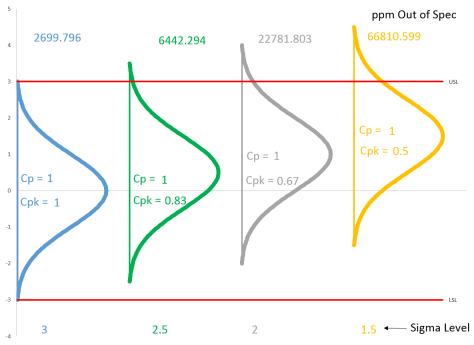
\includegraphics[height=0.3\textheight]{art/Cpk_same_sigma_varying_avg}
\caption[$\cpk$ and $\cp$]{$\cpk$ and $\cp$. \newline
\url{https://www.spcforexcel.com/knowledge/process-capability/interactive-look-process-capability}.}
\label{fig:cpk}
\end{figure}



The $\cpk$ index is motivated by conserving the relation between the index and the non-compliance rate $\pnc$, which is not captured by $\cp$ when the process is not centred. 
Indeed if $\cp$ can be interpreted as ``accuracy compared to a (centred) 3-sigma process'', then $\cpk$ can be interpreted as ``accuracy compared to a (non-centred) 3-sigma process''.
The 3-sigma process is used as a benchmark for historical reasons. 
In practice, it is actually very common to report the sigma-level as a capability index: $\min\set{\frac{USL-\mu}{\sigma},\frac{\mu-LSL}{\sigma}}$, which can be seen as PCR with respect to a 1-sigma process.
Three-sigma would thus be reported as $3$, 6-sigma as $6$, etc.


Another index, known as $\cpm$, or the \emph{Taguchi capability index}, also deals with the non centring but slightly differently. \marginnote{Taguchi Index}
It is motivated by the observation that for $\ctqExpect=\targetValue$, then $\sigma=\sqrt{\expect{(CTQ-\targetValue)^2}}$. This relation does not hold if $\ctqExpect \not=\targetValue$, which leads us to the following definition:
\begin{definition}[$\cpm$]
\begin{align}
		\cpm &:= \frac{USL-LSL}{6 \sqrt{\expect{(CTQ-\targetValue)^2}}} \\
		&= 	\frac{USL-LSL}{6 \sqrt{\sigma^2+(\ctqExpect-\targetValue)^2}} \\ 
		&= \frac{\cp}{\sqrt{1+(\frac{\ctqExpect-\targetValue}{\sigma})^2}}. \label{eq:cpm}
\end{align}
\end{definition}
Eq.(\ref{eq:cpm}) readily shows that just like the $\cpk$, then $\cpm \leq \cp$. 








\subsection{Interval Estimation for Capability Indexes}
Since the various process capability indexes are merely population parameters, we can also construct confidence intervals (CIs) for them, which are very important for small sample sizes, thus point estimates unreliable.
The simplest case is that of $\cp$. Being a monotone transformation of $\sigma$, we can call upon confidence intervals for the variance of a normal population, so that with probability $1-\alpha$:
\begin{align}
\label{eq:ci_for_cp}
	\cp \in \left[ 
		\cpHat \sqrt{\frac{\chi^2_{\alpha/2,n-1}}{n-1}},
		\cpHat \sqrt{\frac{\chi^2_{1-\alpha/2,n-1}}{n-1}}
	\right],
\end{align}
where $\cpHat = \frac{USL-LSL}{6 s}$.
This equation is simply derived from Eq.(\ref{eq:cp_dist}).
Intervals for the other capability indexes, are available in \cite{montgomery_introduction_2007} and references therein. 




\subsection{Testing Hypotheses on Capability}
Consider a supply contract, which requires production to have $\cp>1.5$. 
It may easily be the case, that $\cp>1.5$, even if $\cpHat<1.5$, especially if the sample size is small.
It thus makes a lot of sense, to design hypothesis tests on process capabilities. 
We observe that for an i.i.d. sample from a Gaussian population, where $\cpHat$ is estimated with $s$, then
\begin{align}
\label{eq:cp_dist}
	(n-1) \left( \frac{\cp}{\cpHat} \right)^2  \sim \chi^2_{n-1},
\end{align} 
so that $(n-1) \left( \frac{\cp}{\cpHat} \right)^2 $ may serve as test statistic.

\begin{example}[$\cp$ test for 6-sigma compliance]
\begin{align*}
	H_0: \cp &\leq 2	\\
	H_1:\cp &> 2 \\
	(n-1) \left( \frac{2}{\cpHat} \right)^2  &\overset{H_0}{\sim} \chi^2_{n-1}
\end{align*}
so that the $1-\alpha$ rejection region in $\cpHat$ scale is 
\begin{align*}
	\cpHat > \sqrt{\frac{4 (n-1)}{\chi^2_{n-1,\alpha}}} .
\end{align*}
\end{example}
Note that we should not be testing this hypothesis with the confidence interval in Eq.(\ref{eq:ci_for_cp}) because this particular hypothesis is directional.
Now for a more general case:
\begin{align*}
	H_0: \cp \leq a; 
	H_1:\cp > a 
	&\Rightarrow \text{reject if } \cpHat > \sqrt{\frac{a^2 (n-1)}{\chi^2_{n-1,\alpha}}},\\
	H_0: \cp \geq  a; 
	H_1:\cp < a 
	&\Rightarrow \text{reject if } \cpHat < \sqrt{\frac{a^2 (n-1)}{\chi^2_{n-1,1-\alpha}}}, \\
	H_0: \cp =  a; 
	H_1:\cp \neq a 
	&\Rightarrow \text{reject if } \cpHat < \sqrt{\frac{a^2 (n-1)}{\chi^2_{n-1,1-\alpha/2}}}
	\text{ or } \cpHat > \sqrt{\frac{a^2 (n-1)}{\chi^2_{n-1,\alpha/2}}} \\
\end{align*}














\subsection{Process Performance Indices}
Process \emph{performance} indices measure compliance to specification of a process out of statistical control. 
These include the $\pp$ and $\ppk$ indices. 
Besides mentioning their existence, we will not give them further attention, since we adopt \cite{montgomery_introduction_2007}'s view that their use is strongly discouraged. 


\begin{remark}
At this point, I hope you are wondering why isn't $\pnc$ used as a capability index. 
Well, it is! 
It is simply not called a ``capability index'', simply because the term is reserved to $\cp, \cpk, \cpm$ etc.
\end{remark}



\section{Bibliographic Notes}
This chapter is based almost entirely on \cite{montgomery_introduction_2007}.